\section{Experiments}
\label{sec:exp}
\subsection{Worlds: real LLM outcomes on MMLU-Pro}
We use MMLU-Pro \citep{wang2024mmlupro} (test split, pinned revision; 10-option multiple choice) and open-weight instruction models (Qwen2.5-0.5B/1.5B-Instruct \citep{qwen2025qwen25} here, SmolLM2-1.7B-Instruct in \cref{app:worlds}), scored by the next-token log-probabilities of the option letters after an answer prefix (deterministic; no sampling noise, so all randomness is in the question sample). The pool is a seeded random sample of $N{=}750$ questions among those of at most 200 tokens (65\% of the benchmark; chosen to fit the CPU budget). Three \emph{worlds} (\cref{tab:worlds}; further ones below) supply $Y\in\{0,1\}^{K\times 750}$: \textbf{A}: Qwen2.5-1.5B with $K{=}40$ prompts (8 instructions $\times$ 5 demonstration sets of 0 or 3 validation items); \textbf{B}: Qwen2.5-0.5B with $K{=}40$ configurations (5 prompt formats $\times$ 4 demonstration conditions incl.\ label-biased and 8-shot $\times$ 2 instructions); \textbf{A$\cup$B}: both, $K{=}80$. World A is the practically common regime of a competent model whose accuracy barely depends on the prompt: the 40 configurations span $29.2$--$32.3\%$ and their differences are not reproducible across question halves (split-half reliability $-0.02$), so a \emph{true} improvement from tuning is essentially absent. World B has real structure (raw prompts beat chat formats by 2--6 points; reliability $0.66$) at a near-chance accuracy level; A$\cup$B mixes two very different quality levels (reliability $0.97$). Each episode draws $n\in\{25,\dots,800\}$ questions i.i.d.\ from the pool, runs one optimizer, and applies all protocols; we use $R{=}2000$ episodes per cell (Monte-Carlo s.e.\ of a coverage $\le1$ point; $\pm$ in tables are 95\% intervals).
\begin{table}[t]
\caption{Worlds. Accuracy in \%; sd = standard deviation of true configuration accuracies (points); $\bar\rho$ = mean pairwise correlation of per-question outcomes between configurations; reliability = correlation of configuration accuracies between two random question halves.}\label{tab:worlds}
\centering\scriptsize\setlength{\tabcolsep}{3pt}
\begin{tabular}{lrrrrrr}\toprule
World & $K$ & mean & range & sd & $\bar\rho$ & reliab. \\\midrule
A: Qwen2.5-1.5B, prompt/demo grid ($K{=}40$) & 40 & 30.9 & 29.2--32.3 & 0.72 & 0.79 & -0.02 \\
B: Qwen2.5-0.5B, format/demo grid ($K{=}40$) & 40 & 15.1 & 11.9--19.2 & 2.16 & 0.33 & 0.66 \\
A$\cup$B: union ($K{=}80$) & 80 & 23.0 & 11.9--32.3 & 8.05 & 0.37 & 0.97 \\
\bottomrule
\end{tabular}

\end{table}

\subsection{How far do reported scores overstate true accuracy?}
\begin{figure*}[t]\centering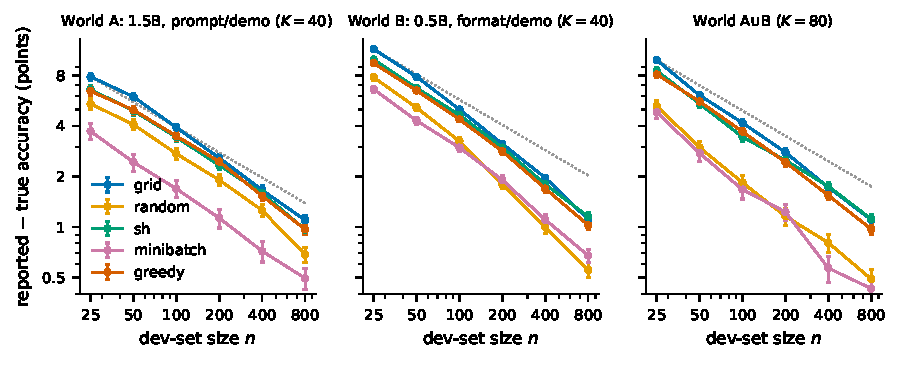
\includegraphics[width=\textwidth]{figs/gap_vs_n.pdf}
\caption{Reported (dev-set) minus true accuracy of the selected configuration against dev-set size, per optimizer (mean over $R{=}2000$ episodes, 95\% CI). Dotted: $n^{-1/2}$ reference through the exhaustive-search point at $n{=}25$.}\label{fig:gap}\end{figure*}
\textbf{Sizeable and slowly shrinking.} With exhaustive search over $K{=}40$ configurations and a dev set of $n{=}100$ questions the reported accuracy exceeds the true accuracy of the deployed configuration by $3.9$ (A), $5.0$ (B) and $4.2$ (A$\cup$B) points, i.e.\ 13\%, 33\% and 18\% relative (\cref{fig:gap}, \cref{tab:gap}); at $n{=}400$ it is still $1.7$, $2.0$, $1.7$. The decay is $n^{-0.57\dots-0.64}$ (log-log slope over $n\le400$), not faster than the $n^{-1/2}$ of \cref{prop:opt}. The overshoot is not merely a small bias: at $n{=}100$ the reported score exceeds the true accuracy of the \emph{best} configuration in the whole search space in 74\%, 83\% and 75\% of episodes (74--90\% over all five worlds), and the 95\% Wilson interval that one would attach to a fixed configuration covers the deployed configuration's accuracy only 88\%, 74\% and 86\% of the time (74--88\% over five worlds). \textbf{All optimizers inflate}, in proportion to how much they look at the dev set: minibatch (MIPRO-like) search and random-8 have the smallest gaps ($1.7/3.0/1.7$ and $2.7/3.2/1.8$ at $n{=}100$) and exhaustive search the largest. \cref{fig:effort} shows this dose--response directly: across optimizer settings the gap grows with the number of full-dev-set passes while the regret (how far $\theta_{\khat}$ is below the best configuration) improves by only $0.4$ points (A) and $2.4$ points (B) between a single configuration and the full grid, while the gap grows by $4$--$5$ points; much of the extra search effort buys optimism rather than accuracy (in A$\cup$B the gain in regret is large only for the first few configurations).
\begin{table}[t]
\caption{Reported $-$ true accuracy (points, mean $\pm$ 95\% CI) by optimizer and dev-set size $n$.}\label{tab:gap}
\centering\scriptsize\setlength{\tabcolsep}{3pt}
\begin{tabular}{lrrrr}\toprule
 & $n{=}50$ & 100 & 200 & 400 \\\midrule
\multicolumn{5}{l}{\emph{A: Qwen2.5-1.5B, prompt/demo grid ($K{=}40$)}} \\
Exhaustive & 6.0$\pm$0.3 & 3.9$\pm$0.2 & 2.6$\pm$0.1 & 1.7$\pm$0.1 \\
Random-8 & 4.1$\pm$0.3 & 2.7$\pm$0.2 & 1.9$\pm$0.1 & 1.3$\pm$0.1 \\
Succ. halving & 4.9$\pm$0.3 & 3.4$\pm$0.2 & 2.3$\pm$0.1 & 1.6$\pm$0.1 \\
Minibatch (MIPRO-like) & 2.4$\pm$0.3 & 1.7$\pm$0.2 & 1.1$\pm$0.1 & 0.7$\pm$0.1 \\
Greedy coord. & 5.0$\pm$0.3 & 3.5$\pm$0.2 & 2.5$\pm$0.1 & 1.5$\pm$0.1 \\
\multicolumn{5}{l}{\emph{B: Qwen2.5-0.5B, format/demo grid ($K{=}40$)}} \\
Exhaustive & 7.8$\pm$0.2 & 5.0$\pm$0.1 & 3.1$\pm$0.1 & 2.0$\pm$0.1 \\
Random-8 & 5.1$\pm$0.2 & 3.2$\pm$0.1 & 1.8$\pm$0.1 & 1.0$\pm$0.1 \\
Succ. halving & 6.7$\pm$0.2 & 4.6$\pm$0.1 & 3.0$\pm$0.1 & 1.8$\pm$0.1 \\
Minibatch (MIPRO-like) & 4.3$\pm$0.2 & 3.0$\pm$0.2 & 1.9$\pm$0.1 & 1.1$\pm$0.1 \\
Greedy coord. & 6.5$\pm$0.2 & 4.4$\pm$0.1 & 2.8$\pm$0.1 & 1.7$\pm$0.1 \\
\multicolumn{5}{l}{\emph{A$\cup$B: union ($K{=}80$)}} \\
Exhaustive & 6.1$\pm$0.3 & 4.2$\pm$0.2 & 2.8$\pm$0.1 & 1.7$\pm$0.1 \\
Random-8 & 3.0$\pm$0.3 & 1.8$\pm$0.2 & 1.2$\pm$0.1 & 0.8$\pm$0.1 \\
Succ. halving & 5.4$\pm$0.3 & 3.4$\pm$0.2 & 2.5$\pm$0.1 & 1.7$\pm$0.1 \\
Minibatch (MIPRO-like) & 2.7$\pm$0.3 & 1.7$\pm$0.2 & 1.2$\pm$0.1 & 0.6$\pm$0.1 \\
Greedy coord. & 5.6$\pm$0.3 & 3.7$\pm$0.2 & 2.4$\pm$0.1 & 1.5$\pm$0.1 \\
\bottomrule
\end{tabular}

\end{table}
\begin{figure*}[t]\centering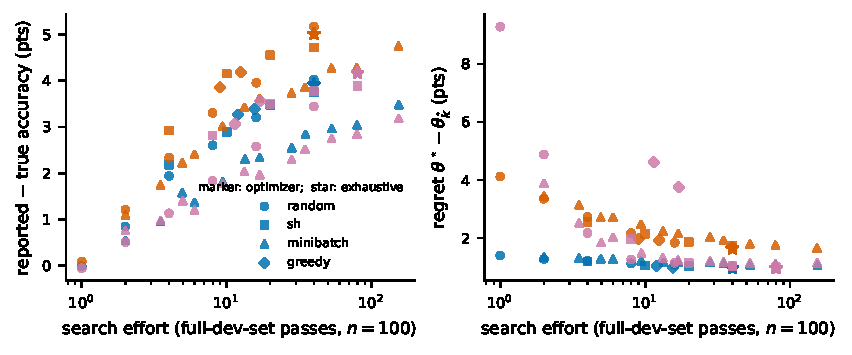
\includegraphics[width=.92\textwidth]{figs/search_effort.pdf}
\caption{Search effort vs.\ optimism (left) and regret (right), $n{=}100$; colours: worlds (blue A, orange B, pink A$\cup$B), markers: optimizer settings (random $B\in\{1,\dots,40\}$, SH budget, minibatch trials $\times$ minibatch size, greedy); stars: exhaustive.}\label{fig:effort}\end{figure*}

\subsection{What drives the gap}
\begin{figure*}[t]\centering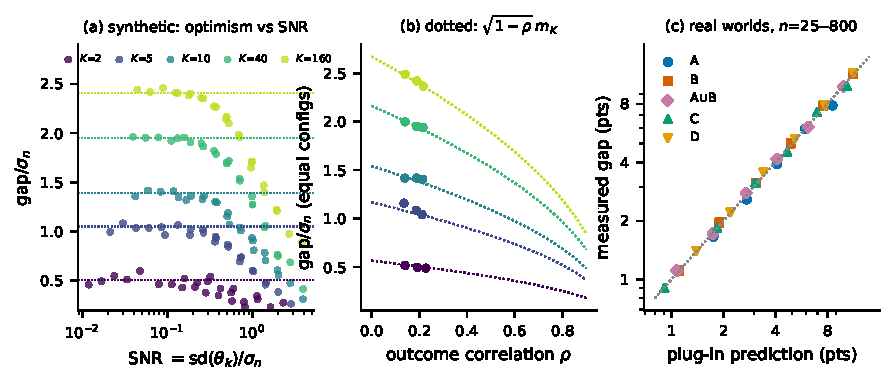
\includegraphics[width=\textwidth]{figs/theory_check.pdf}
\caption{(a,b) Synthetic worlds: optimism in units of $\sigma_n$ depends on the number of configurations $K$, their outcome correlation $\rho$, and the signal-to-noise ratio $\mathrm{sd}(\theta_k)/\sigma_n$; dotted: $\sqrt{1-\rho}\,m_K$ of \cref{prop:opt}(c). (c) Real worlds: Gaussian plug-in prediction (dev means $\sim N(\theta,\mathrm{Cov}(Y)/n)$, true $\theta$, Cov from the pool) vs.\ measured optimism of exhaustive search, all $n$.}\label{fig:theory}\end{figure*}
\cref{fig:theory}(a,b) confirm \cref{prop:opt}(c) on synthetic worlds: for equally good configurations the normalised optimism equals $\sqrt{1-\rho}\,m_K$ to within the plotting resolution, and it falls with $\mathrm{SNR}=\mathrm{sd}(\theta_k)/\sigma_n$ once the best configuration becomes identifiable. On the real worlds a Gaussian plug-in that uses the pool's $\theta$ and outcome covariance predicts the measured optimism of exhaustive search within $9.2\%$ (mean $2.6\%$) for all 30 (world, $n$) cells of the five worlds (\cref{fig:theory}c; the figure marks A, B, A$\cup$B, C, D), so the mechanism is the maximum of correlated, approximately Gaussian estimation errors. Practical consequences: (i) \emph{number of effectively distinct configurations}, not nominal $K$, matters---world A has $\bar\rho{=}0.79$ and a gap of $3.9$ points, world B ($\bar\rho{=}0.33$) $5.0$ at lower accuracy; (ii) the gap is governed by $\sigma_n=\sqrt{p(1-p)/n}$, so it is largest relative to accuracy for hard benchmarks and small $n$; (iii) \cref{fig:ksweep} (appendix) shows that the gap grows roughly like $\sqrt{\ln K}$ with the number of configurations searched.

\subsection{Effect on conclusions drawn from reported scores}
\begin{figure*}[t]\centering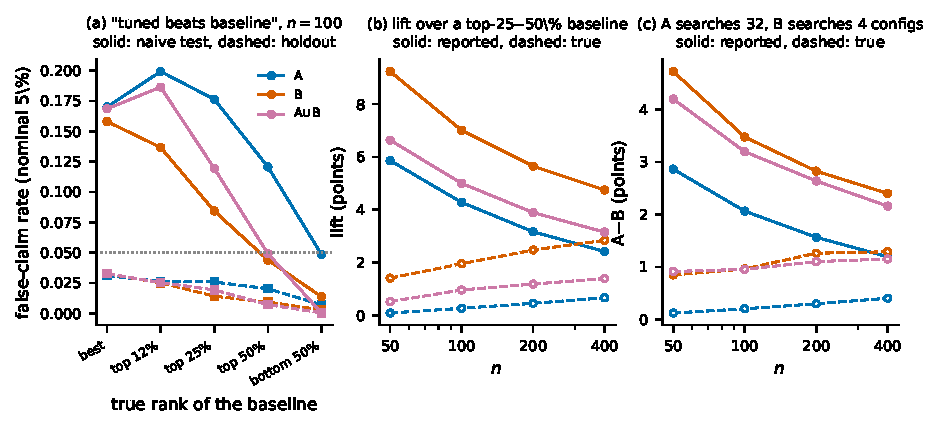
\includegraphics[width=\textwidth]{figs/conclusions.pdf}
\caption{Consequences. (a) A paired one-sided test (nominal 5\%) that the tuned system beats a baseline configuration, as a function of the baseline's true rank in the space: fraction of \emph{false} claims (claim made while the true lift is $\le0$) with the naive test (solid) and with a 50/50 holdout (dashed). (b) Reported vs.\ true lift over a baseline from the 25--50\% quantile. (c) System A tuned over 32 configurations vs.\ system B tuned over 4 (disjoint, random); reported vs.\ true difference.}\label{fig:concl}\end{figure*}
\textbf{Lifts over a baseline.} A natural claim is ``automatic tuning improved accuracy by $\delta$ over the baseline prompt''. If the baseline is already a good configuration (top 12\% of the space), the one-sided paired test on the dev set declares a significant improvement in $19$/$14$/$18\%$ of episodes at $n{=}100$ (A/B/A$\cup$B) although tuning cannot help; the 50/50 holdout test errs in $3\%$. For a mid-ranked baseline (true rank in the top 25--50\%) the reported lift at $n{=}100$ is $4.3/7.0/5.0$ points versus true lifts of $0.3/2.0/1.0$ (\cref{tab:concl}, \cref{fig:concl}b)---in world A tuning delivers nothing measurable although the average episode ``finds'' a multi-point gain. \textbf{Comparing systems tuned with different budgets.} If system A searches 32 configurations and B searches 4 on the same dev set, the reported advantage of A is $2.1/3.5/3.2$ points versus a true advantage of $0.2/1.0/1.0$ (A/B/A$\cup$B, $n{=}100$): a 3--10$\times$ inflation (\cref{prop:cmp}); the holdout comparison is unbiased for the selected pair ($0.0/0.9/0.9$).
\begin{table}[t]
\caption{Claims at $n$ questions ($K_A{=}32$ vs $K_B{=}4$ in the last columns). False-claim rate: baseline in the top 12\% of the space, nominal 5\%. Lift: baseline of true rank 11--20 of $K$ (top 25--50\%), reported / true (points); `holdout lift' is the 50/50 holdout estimate. A$-$B: reported / true (points) and holdout estimate.}\label{tab:concl}
\centering\scriptsize\setlength{\tabcolsep}{2.5pt}
\begin{tabular}{rrrrrrr}\toprule
$n$ & false claim & (holdout) & lift & holdout lift & A$-$B & (holdout) \\\midrule
\multicolumn{7}{l}{\emph{A: Qwen2.5-1.5B, prompt/demo grid ($K{=}40$)}} \\
50 & 0.22 & 0.02 & 5.9 / 0.1 & -0.1 & 2.9 / 0.1 & -0.1 \\
100 & 0.19 & 0.03 & 4.3 / 0.3 & 0.1 & 2.1 / 0.2 & 0.0 \\
200 & 0.14 & 0.02 & 3.2 / 0.5 & 0.3 & 1.6 / 0.3 & 0.2 \\
400 & 0.10 & 0.02 & 2.4 / 0.7 & 0.4 & 1.2 / 0.4 & 0.3 \\
\multicolumn{7}{l}{\emph{B: Qwen2.5-0.5B, format/demo grid ($K{=}40$)}} \\
50 & 0.18 & 0.02 & 9.2 / 1.4 & 0.9 & 4.7 / 0.8 & 0.7 \\
100 & 0.14 & 0.03 & 7.0 / 2.0 & 1.4 & 3.5 / 1.0 & 0.9 \\
200 & 0.11 & 0.02 & 5.6 / 2.5 & 2.0 & 2.8 / 1.3 & 1.0 \\
400 & 0.07 & 0.01 & 4.7 / 2.8 & 2.4 & 2.4 / 1.3 & 1.2 \\
\multicolumn{7}{l}{\emph{A$\cup$B: union ($K{=}80$)}} \\
50 & 0.20 & 0.02 & 6.6 / 0.5 & -0.8 & 4.2 / 0.9 & 0.6 \\
100 & 0.18 & 0.03 & 5.0 / 1.0 & 0.5 & 3.2 / 1.0 & 0.9 \\
200 & 0.13 & 0.02 & 3.9 / 1.2 & 1.0 & 2.6 / 1.1 & 1.0 \\
400 & 0.10 & 0.02 & 3.2 / 1.4 & 1.2 & 2.2 / 1.1 & 1.0 \\
\bottomrule
\end{tabular}

\end{table}

\subsection{Reporting protocols}
\begin{table*}[t]
\caption{Reporting protocols, exhaustive search, $n{=}100$, $R{=}2000$ episodes. Bias and RMSE of the estimate of the deployed configuration's true accuracy (points; for holdout the target is the accuracy of the holdout-selected configuration), coverage and mean width (points) of the nominal 95\% interval; s.e.\ of bias $\le0.4$, of coverage $\le1$ point. Max-$t$ is centred at the naive score; empirical Bayes uses the recentred interval.}\label{tab:proto}
\centering\scriptsize\setlength{\tabcolsep}{4pt}
\begin{tabular}{lrrrr}\toprule
Protocol & bias & RMSE & coverage & width \\\midrule
\multicolumn{5}{l}{\emph{A: Qwen2.5-1.5B, prompt/demo grid ($K{=}40$)}} \\
Naive (dev score) & +3.9 & 5.8 & 0.88 & 18.3 \\
Holdout split (50/50) & +0.0 & 6.4 & 0.95 & 24.6 \\
5-fold cross-fit & -0.2 & 5.1 & -- & -- \\
Replay bootstrap (opt.) & +1.1 & 4.6 & -- & -- \\
Replay bootstrap (.632) & +1.3 & 4.6 & -- & -- \\
Empirical Bayes & +0.1 & 4.3 & 0.96 & 18.7 \\
Max-t simultaneous & +3.9 & 5.8 & 0.98 & 25.6 \\
Conditional (winner) & -8.7 & 18.3 & 0.72 & 21.9 \\
Ladder ($n^{-1/2}$) & +0.2 & 5.0 & -- & -- \\
\multicolumn{5}{l}{\emph{B: Qwen2.5-0.5B, format/demo grid ($K{=}40$)}} \\
Naive (dev score) & +5.0 & 5.9 & 0.74 & 16.1 \\
Holdout split (50/50) & +0.1 & 5.3 & 0.95 & 20.3 \\
5-fold cross-fit & -0.3 & 4.8 & -- & -- \\
Replay bootstrap (opt.) & +1.0 & 3.7 & -- & -- \\
Replay bootstrap (.632) & +1.5 & 3.7 & -- & -- \\
Empirical Bayes & -0.3 & 3.3 & 0.98 & 15.6 \\
Max-t simultaneous & +5.0 & 5.9 & 1.00 & 25.4 \\
Conditional (winner) & -3.1 & 9.6 & 0.82 & 22.1 \\
Ladder ($n^{-1/2}$) & +1.9 & 4.5 & -- & -- \\
\multicolumn{5}{l}{\emph{A$\cup$B: union ($K{=}80$)}} \\
Naive (dev score) & +4.2 & 6.0 & 0.86 & 18.4 \\
Holdout split (50/50) & -0.1 & 6.5 & 0.95 & 24.5 \\
5-fold cross-fit & +0.1 & 5.2 & -- & -- \\
Replay bootstrap (opt.) & +1.2 & 4.8 & -- & -- \\
Replay bootstrap (.632) & +1.3 & 4.7 & -- & -- \\
Empirical Bayes & +2.3 & 5.2 & 0.88 & 16.0 \\
Max-t simultaneous & +4.2 & 6.0 & 0.99 & 30.0 \\
Conditional (winner) & -7.8 & 17.8 & 0.73 & 22.5 \\
Ladder ($n^{-1/2}$) & +0.7 & 5.2 & -- & -- \\
\bottomrule
\end{tabular}

\end{table*}
\begin{figure}[t]\centering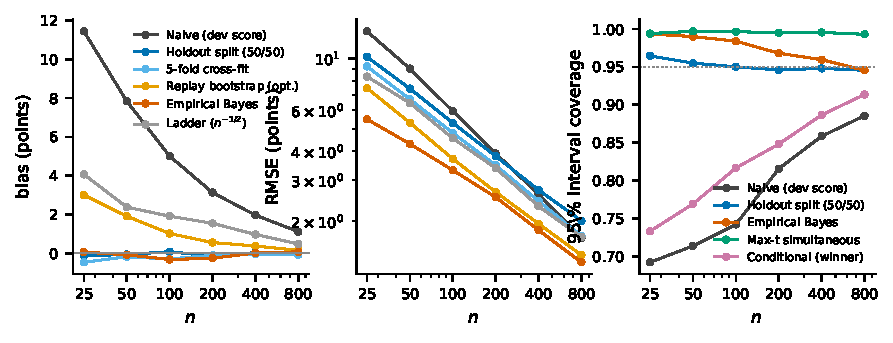
\includegraphics[width=\columnwidth]{figs/protocols_b05.pdf}
\caption{Bias, RMSE and coverage of the protocols against $n$, exhaustive search, world B (other worlds in \cref{fig:protocols}).}\label{fig:proto_b}\end{figure}
\textbf{Sample splitting} (P2) is unbiased with exact 95\% coverage in every world, but is not accurate: its RMSE is $5.3$--$6.5$ points at $n{=}100$ (no better than the naive score in A and A$\cup$B, because discarding half of the questions doubles the sampling variance of the score), its interval is wider than the naive one ($20$--$25$ vs.\ $16$--$18$ points), and it deploys a worse configuration ($-0.16/-0.55/-0.45$ points at $f{=}0.5$; up to $-1.3$ at $f{=}0.3$; \cref{tab:split}). Cross-fitting (P3) has low bias for the procedure but cannot attach an interval to the specific $\khat$. The \textbf{search-replay bootstrap} (P4) removes $70$--$80\%$ of the optimism for exhaustive search (at $n{=}100$ residual bias $+1.1/+1.0/+1.2$ vs.\ $+3.9/+5.0/+4.2$; RMSE $4.6/3.7/4.8$, lower than splitting). The \textbf{empirical-Bayes} correction (P5) is the most accurate dev-set-only method when configurations look exchangeable (A: bias $+0.1$, RMSE $4.3$; B: $-0.3$, $3.3$; recentred interval coverage $0.96$/$0.98$ at the width of the naive interval), but it \emph{fails when the prior is not roughly normal}: in A$\cup$B (two quality clusters) its bias is $+2.3$ and coverage $0.88$, and it requires scoring all configurations on all of $D$. \textbf{Max-$t$} (P6) is conservative but always valid for exhaustive/random search (coverage $\ge0.98$; width $25$--$30$ points vs.\ $16$--$18$ for naive); its point estimate is the biased naive score. The \textbf{conditional winner} interval (P7) is poorly calibrated for discrete accuracies (coverage $0.72$--$0.82$, RMSE $9.6$--$18$ points) although our implementation attains $95.4\%$ coverage on continuous Gaussian data (\texttt{code/check\_cond.py}), i.e.\ the Gaussian/ties approximation, not the principle, is at fault. The \textbf{Ladder} (P8) is nearly unbiased only where nothing is really better (A) because it rarely moves off its starting configuration; in B it deploys $1.1$ points less accuracy than exhaustive search and still reports $+1.9$ too high. Appendix tables repeat the comparison for all optimizers (replay bootstrap and, heuristically, empirical Bayes remain reasonably accurate for minibatch and greedy search) and $n$.

\begin{table}[t]
\caption{Cost and accuracy of sample splitting, exhaustive search, $n{=}100$. `cost' = loss in true accuracy of the deployed configuration relative to selecting with all $n$ (points).}\label{tab:split}
\centering\scriptsize\setlength{\tabcolsep}{3pt}
\begin{tabular}{lrrrrr}\toprule
Protocol & cost & bias & RMSE & cover. & width \\\midrule
\multicolumn{6}{l}{\emph{A: Qwen2.5-1.5B, prompt/demo grid ($K{=}40$)}} \\
no split (naive) & 0.0 & +3.9 & 5.8 & 0.88 & 18.3 \\
select on 30\% / report on 70\% & 0.27 & -0.1 & 5.4 & 0.96 & 21.0 \\
select on 50\% / report on 50\% & 0.16 & +0.0 & 6.4 & 0.95 & 24.6 \\
select on 70\% / report on 30\% & 0.09 & +0.1 & 8.4 & 0.95 & 31.0 \\
\multicolumn{6}{l}{\emph{B: Qwen2.5-0.5B, format/demo grid ($K{=}40$)}} \\
no split (naive) & 0.0 & +5.0 & 5.9 & 0.74 & 16.1 \\
select on 30\% / report on 70\% & 1.00 & -0.0 & 4.6 & 0.94 & 17.0 \\
select on 50\% / report on 50\% & 0.55 & +0.1 & 5.3 & 0.95 & 20.3 \\
select on 70\% / report on 30\% & 0.32 & -0.1 & 6.8 & 0.95 & 25.8 \\
\multicolumn{6}{l}{\emph{A$\cup$B: union ($K{=}80$)}} \\
no split (naive) & 0.0 & +4.2 & 6.0 & 0.86 & 18.4 \\
select on 30\% / report on 70\% & 1.26 & +0.0 & 5.5 & 0.95 & 20.8 \\
select on 50\% / report on 50\% & 0.45 & -0.1 & 6.5 & 0.95 & 24.5 \\
select on 70\% / report on 30\% & 0.16 & -0.2 & 8.3 & 0.95 & 30.9 \\
\bottomrule
\end{tabular}

\end{table}
